\chapter{Supplementary Result Figures}
\label{app:supplementary}

This appendix collects supplementary figures referenced from Chapter~\ref{chap:experiments}. They support the main results but are not central to the argument, so they are placed here to keep the experiments chapter focused.

\begin{figure}[htbp]
\centering
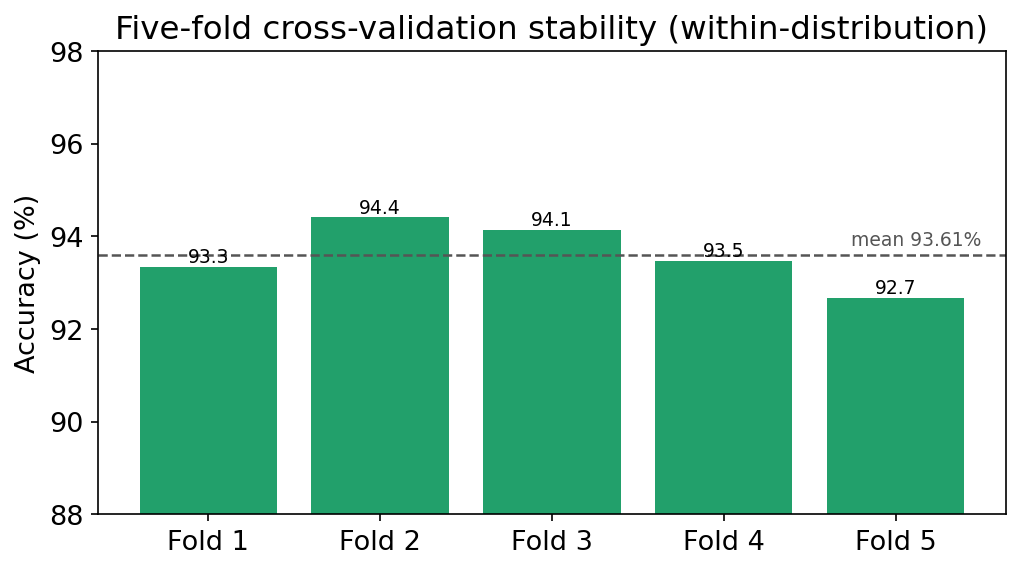
\includegraphics[width=0.92\textwidth]{figures/Figure_7_5_fivefold_stability.png}
\caption[Per-fold accuracy under five-fold cross-validation on Garmin...]{Per-fold accuracy under five-fold cross-validation on Garmin users~1--6. The low variance across folds shows the within-distribution result is stable and not driven by a single favorable split.}
\label{fig:ch7_fivefold_stability}
\end{figure}

\begin{figure}[htbp]
\centering
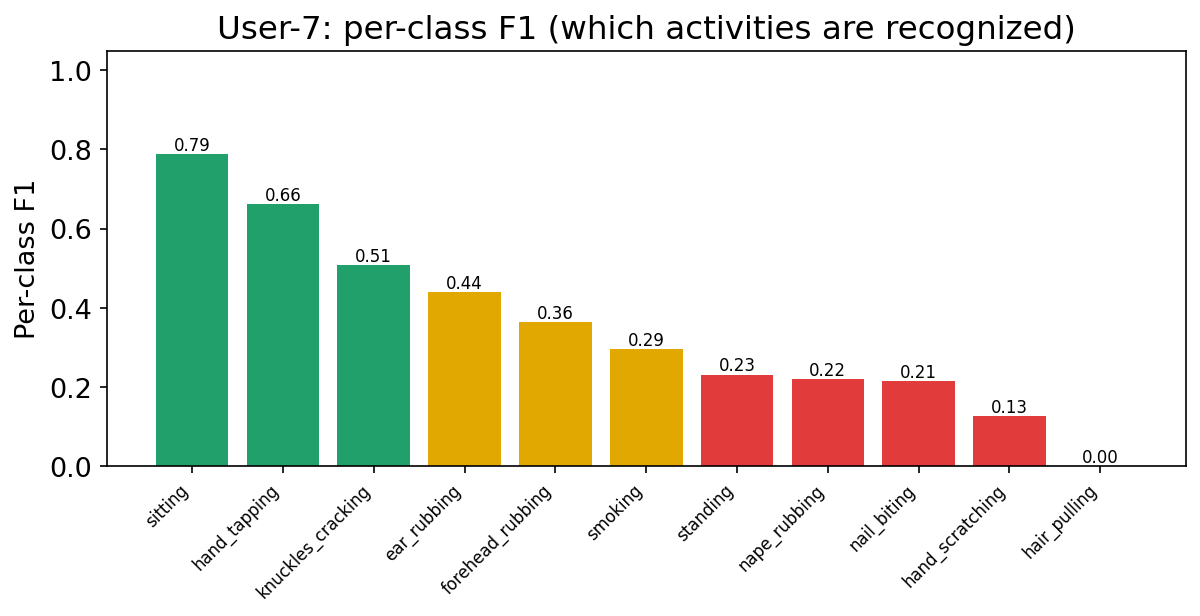
\includegraphics[width=0.92\textwidth]{figures/Figure_7_6_user7_per_class.png}
\caption[Per-class F1 on the blind User~7 probe]{Per-class F1 on the blind User~7 probe. Recognition is highly uneven across the eleven activities: a few activities such as hand tapping are recognized reliably while several fine-grained behaviors receive an F1 close to zero. The macro-averaged F1 of 0.350 summarizes this spread.}
\label{fig:ch7_user7_perclass}
\end{figure}

